% !TeX root = main.tex
\chapter{Paper-based semantic speech editing}\label{chp:paper}

% Need for paper
One of the findings from Chapter~\ref{chp:screen} was that some producers find their work environment noisy and
distracting, and do not like working with screens for extended periods. This leads many to print out transcripts of
speech recordings so that they can review and edit the recordings away from the screen and/or office.

% Advantage of paper
Working on paper offers a number of advantages over working on screens. Most of these are self-evident, but still
worth reviewing.  Paper is lightweight, portable and does not require any power, which allows users to work almost
anywhere.  It is not back-lit, so is easier on the eyes.  It can be navigated quickly, annotated freely whilst reading,
and individual pages can be laid out and easily compared.  Its physical low-tech nature also means that it is
intuitive, robust, durable and does not crash or lose data.  Reading from paper rather than a screen allows readers to
gain a deeper understanding, easily cross-reference other documents, and interleave reading and writing
\citep{OHara1997,Mangen2013,Singer2017}.

%Transcripts are often printed out because:
%- it is easier to read than on screen
%- allows portability,
%- allows annotation,
%- flexible spatial layout
%- quick navigation
%- cross-referencing,
%- reduces battery anxiety,
%- more trusted by non-tech-savvy users

%A similar process happens in the production of media content. The production workflow typically involves recording
%material, selecting which parts of that material to use, then editing the desired material down to the final output
%\citep{Baume2015}.  Many producers will `log' the material after it is recorded by writing transcripts of what was
%said.  This is either done themselves or using a third-party service. These transcripts help producers to recall what
%was said and when, identify themes, and make links between different parts of their content.

% Disadvantage of paper
Compared to digital media, working with a physical medium like paper introduces restrictions that make it more
difficult to copy, share, store and archive information. Printing a document breaks the link to its digital source, so
is normally a one-way process, where any information that is changed/added cannot is not fed back. Additionally,
freehand annotations are unstructured, and cannot easily be digitised and re-used. This forces users to manually
re-enter the information into a computer. In the case of radio production, this involves using a DAW to edit the audio
based on paper notes, which can be slow and tedious.

% Digital paper
There are a number of technological solutions that can be used to create a `digital bridge' between paper and
its digital source. These offer the possibility to combine the advantages of paper and digital workflows. Using this
approach, it is possible to link the words on a printed transcript of speech to the time they were spoken in the
original audio recording. Furthermore, by linking the paper annotations to audio edit commands, the paper could be used
to directly edit the audio content.

% Intro
In this chapter, we investigate paper-based workflows in the context of professional radio production. We describe how
we captured the requirements for a paper-based speech editor, and how we designed and built a working prototype. We
then describe a contextual study of radio production in which we directly compared screen-based and paper-based
workflows. 

\section{Background}\label{sec:paper-background}
Radio production using a paper interface requires a system that automatically translates annotations on a printed
transcript to audio edit commands. Such a system requires a method of linking paper to media.

`The Audio Notebook' \citep{Stifelman2001} was a system that used a physical pen and paper interface in combination
with a device that recorded audio synchronously with the page and vertical location of the written notes.  The device
could also replay the audio from a page and display which notes relate to the current playback position using an LED
scrollbar display at the side of the page. Users could also use the scrollbar to control the position of the audio
playback.  A longitudinal study of six participants over five months again found that users needed to take fewer notes,
and made more notes during replay. Two of the participants were reporters who used the system while recording
interviews. One reporter made minimal notes during the interview, but replayed the interview and made additional notes,
including star symbols to indicate important moments. They also extracted quotes of interest by typing them into a
computer. The other reporter was skeptical of the system, so made detailed notes so not to rely on the audio. However,
they were later able to use the system to recall bits of the interview, which was many times faster than their existing
technique of fully transcribing the audio recording.

We have identified three main approaches for achieving this, using barcodes, digital ink and digital pens.
In this section, we will review previous systems and studies that have used these techniques to link media with written
documents.

%\subsection{Screen-based}
%Transcript-based interfaces have already successfully been applied to both audio and video editing. SCANMail
%\citep{Whittaker2002} demonstrated the advantages of navigating voicemail recordings using a transcript, but did not
%include editing capabilities.  The LIDS Editor \citep{Apperley2002}, and later TRAED \citep{Masoodian2006}, used
%automatically-generated transcripts to allow users to navigate and edit lecture recordings by removing and rearranging
%sentences and words. Even though automatically-generated transcripts are imperfect, Whittaker and Amento found they are
%sufficiently accurate to allow navigation and editing \citep{Whittaker2004}.  More recently, Rubin \citep{Rubin2013}
%created a system for using editable crowd-sourced transcripts to create audio stories.  Similar techniques have been
%applied to video editing. SILVER \citep{Casares2002} was a video editor that had an editable transcript window,
%generated from subtitles, and Berthouzoz et al.  \citep{Berthouzoz2012} developed a system that used crowd-sourced
%transcripts and image processing to allow text-based editing of multi-camera video interviews.

\subsection{Barcodes}
Paper transcripts have been explored as a method of navigating video recordings by using a device to detect the
position in the text and play the video from that position. \citet{Hull2003} describes a system called `Video Paper',
which embedded video keyframes with barcodes down the side of the page. It used a PDA to scan the barcodes that linked
to a position in a video, which was downloaded and played on the device. \citet{Klemmer2003} applied Video Paper to
oral history in a project called `Books with Voices'. An evaluation of 13 users found that it had substantial benefits
with minimal overhead.  \citet{Erol2007} went a step further by embedding the video in the barcode data, removing the
need to download the video from a separate source. \citet{Erol2008} removed the need for barcodes by creating a system
called `HotPaper', which used a camera to measure the whitespace between words and matched that to unique patterns in
the text.

Barcode-based systems provide a link between text and media, however they do not provide a convenient method of
capturing annotations. It would be possible to use a PDA-style device to capture annotations and link them to a
particular barcode. However, this requires that the annotation are entered into a handheld device, rather that just
written on the paper. Additionally, the size of the barcodes means that the precision of the timestamps would be at a
sentance-level rather than word-level.

\subsection{Digital ink}
`Digital ink' refers to technology that digitally captures and responds to the moments of a pen, such as a stylus on a
tablet PC.

\subsubsection{Synchronised note-taking}
`Marquee' \citep{Weher1994} was a digital ink system for supporting the task of logging during a live video recording.
Users could make synchronised handwritten notes by drawing a horizontal line to mark a timestamp, then writing their
notes below.  Additionally, they could create a list of keywords, and add them to their notes by pressing them at the
right moment.  Marquee was evaluated for note-taking during meetings with three participants. The study found that
users did not partake in discussions while logging, which may prevent such a system being used during an interview.
The freehand nature of the notes meant that it could easily handle the different styles of each user.  Users reported
that they didn't feel they had to make as many notes as they normally would, because they could later refer back to the
video recording. The authors also noted that videos can be further annotated during replay, allowing for an iterative
logging process.

`Dynomite' \citep{Wilcox1997} was a virtual notebook that recorded audio synchronously with digital ink handwritten
notes. The user's notes could be assigned to different `properties', either before or after they were written, to
indicate an action point, for example, or a user-specified keyword.  Users could also highlight a portion of the audio
by pressing a `mark' button or making a specific gesture.  This would highlight the audio for a specified time period,
unless the `extend' or `end mark' buttons were pressed.  Any notes made during this period were displayed in bold and
the highlighted segments were displayed using colours on a horizontal timeline. An evaluation of nine users found that
users took fewer notes when using the audio highlighting, and that they wanted to go back and use the audio to improve
the notes afterwards. Both of these findings mirror those from \citet{Weher1994}.

\subsubsection{Video editing}
Several systems have experimented with using pens with interactive sliders to provide advanced control for
navigating video content, such as `LEAN' \citep{Ramos2003}, `Zlider' \citep{Ramos2005} and MobileZoomSlider/ScrollWheel
\citep{Huerst2008}. However, these systems are limited to the navigation of content, without changing or labelling it.
Our interest is primarily in the annotation and editing of media, which the following systems have explored using
digital ink interfaces.

\citet{Diakopoulos2006} created a digital ink interface for creating and annotating segments of a pre-recorded video,
called `VideoTater'. Segments could be created by drawing a vertical line on a video timeline, and merged by drawing a
horizontal line between them. Each segment could be tagged by selecting it and hand-writing text. The back of
the pen could be used to erase tags. Pen pressure was used to distinguish between selection and tagging, with low
pressure for selecting and high for tagging. Informal feedback from three users found that the gestures were
successful, and that the pressure mapping worked well.

\citet{Cattelan2008} added functionality for marking edit commands using digital ink in their system `WaCTool'. The
system included a variety of features for annotation, editing and real-time collaboration. Users could use a pen to
write annotations by tapping the video to freeze it, then drawing on the video frame.  Users could apply a `skip'
command to a segment of the video by using the pen to tap the bottom left of the video at the start of an unwanted
segment, and tapping the bottom right at the end. The `skip' command is analogous to editing out part of the video.
Similar commands for looping and slow motion were also available by tapping different regions.

`Video as Ink' \citep{Cabral2016} took an alternative approach by allowing users to `paint' video frames and segments
onto a 2D canvas using a pen and tablet interface. The canvas works as a timeline, but extends vertically in both
directions so that the video can be painted onto multiple rows. The system includes gestures for adding, moving,
erasing and selecting content. An evaluation of 12 participants found that the canvas allowed users to creatively
explore different possibilities. However, the interface relies on the visual organisation of images, which does not
necessarily translate well to audio and text.

\subsubsection{Proof-reading}

\citet{Yoon2014} created a collaborative digital ink document annotation system called `RichReview', which offered
users three modalities in which to annotate documents - freeform inking, voice recording and deictic gestures. The
voice recordings were displayed using a waveform, overlaid with an automatically generated transcript of the speech.
Users could trim or tidy the voice recordings by drawing a line through words or pauses to remove them.  The system was
evaluated using a qualitative study of 12 students which found that the editing features were considered easy to use
and efficient for removing `umm's and long pauses.  However, many participants reported that the transcripts were not
accurate enough to use without having to listen to the audio.

\subsection{Digital pens}
A digital pen looks and functions as a normal pen, but includes an on-board infrared camera that tracks the position of
the pen while it writes on paper. Digital pens must be used in combination with paper that has a unique non-repeating
dot pattern printed onto it using a standard colour laser printer.  By reading this pattern, the pen can calculate
exactly where it is when touching the page. This information is captured up to 100 times a second and recorded
digitally onto the pen. Depending on which pen and which software you're using, this information can either be streamed
live via Bluetooth, or downloaded as a batch onto a computer. This technology has been patented by Anoto Group
\citep{Fahraeus2003}, who exclusively manufacture and licence digital pen products. As such, this technology is often
referred to as the `Anoto dot pattern'.

% Pens
%Livescribe Pulse
%Live Pen 1 (DP-201)
%Live Pen 2

\subsubsection{Proof-reading}

\citet{Guimbretiere2003} introduced a concept called `PADD', which was a system of editing documents that uses the
Anoto pattern to allow users to move from digital documents to paper and back again. \citet{Conroy2004} created
`ProofRite', which was the first full implementation of a PADD system. It captured annotations made to a printed text
document, and overlaid the annotations onto the text in a word processor. The annotations were anchored to the text,
such that they `reflow' when the text is moved. Through informal feedback, users suggested that their annotations
should translate into actions such as delete.

\citet{Weibel2008} created `PaperProof', which interpreted the edit annotations and automatically applied them to the
document. Gestures for delete, insert, replace, move and annotate were translated into modifications in a word
processor, and intelligent character recognition was used to digitise any hand-written text. Processing the annotations
allows for a two-way interaction between the digital and paper representations. There were no user studies of the
PaperProof system.

\subsubsection{Synchronised note-taking}

ChronoVis \citep{Fouse2011} used the Anoto dot pattern to record paper notes during playback of a video. The on-screen
playback interface allowed users to click on the digital display of the handwritten notes to navigate to that position
in the video, or browse a list of timestamped notes. Alternatively, they could reprint their notes and use a
wirelessly-connected digital pen to tap on the notes, which controlled the playback position.
ChronoVis can also coordinate multiple data sources, such as GPS logs.

\citet{Weibel2012} conducted a longitudinal study of ChronoViz for use in observational research. They studied how
three research groups used the technology over a period of 18 months by observing their use of ChronoVis, and
conducting regular focus group and brainstorming discussions.  The study found that the introduction of the system
changed the note-taking practices of the participants.  Notes became a mixture of linear notes and symbolic
representations.  Asterisks, stars and simple shapes were used as bookmarks for later referral.  Strokes in certain
areas of the paper were used to capture structured data. Single strokes were used for binary data (like a checkbox),
multiple strokes were used for counting events, and handwriting was used for categorical data.  One research group
stopped manually writing the time as they normally would, because this information was captured automatically. The
flexibility of freehand notes also enabled use of arrows in various contexts such as to indicate direction and actions.

Paper-digital notes introduce time as an additional structuring factor, and the authors discuss the tension between the
use of time and space. They point out that `deciding when time, space or both are important in a paper-digital form is
complex'.  One benefit of a paper-digital interface is that when the digital pen fails, the paper still contains
important information, however this is not true for time information.

Based on feedback from this study, ChronoVis was enhanced with features to control video playback, automatically
recognise specific symbols and add notes on top of existing notes.

% Sensitivity of zones - a line which crosses from one zone to another can be a problem.
% Problems when line or symbols crosses over zone

%\subsection{Synchronised note-taking}
%A number of previous systems have explored how media can be annotated as it is recorded or replayed. These have often
%been developed for note-taking during meetings or lectures, but could also be applied to radio production. Although we
%did not find that it was commmon to write notes during interviews, we found that producers often listen back to their
%recordings, so these systems could be using during that replay process.

%\subsection{Correction}
%In chapter~\ref{chp:screen}, we identified that some producers were interested in correcting the transcript for sharing
%with others, or for later publication.

%TODO There are clearly defined symbols for use in proof correction (e.g. \citet{ISO5776}).

%TODO Interfaces to correct errors in transcripts have also been considered, such as that from \citet{Suhm2001}.

\subsection{Summary}

% MECHANISMS
% - digital ink vs digital pen vs barcode
In this section, we have seen how barcodes, digital ink and digital pens have been used to link written documents to
timed media.

Barcodes provide a simple mechanism for linking physical printed paper to digital media. This provides the
benefits that come with reading from and annotating paper, but with a link to the source media. The barcodes are easy
to generate, don't need a licence and are robust to photocopying.  We need a device to read the barcodes, but we
could do this using the camera on a mobile phone.  The systems to date have only provided a one-way link from paper to
media.  It would be possible to implement a feedback mechanism, but the data would have to be entered into the scanning
device rather than the paper. This means that the freehand annotation are not supported, not would they be accessible
without using the device. Barcodes also take up a lot of space, so it is only practical to have them at the end
of a line, rather than for each word. This limits the precision with which they can be used.

Digital ink interfaces are vastly more feature-rich as they use a device with a screen that is capable of advanced
two-way interaction. The device can integrate with media playback to allow users listen to the audio. Freehand
annotations can be used to annotate documents, and these can easily be undone or erased. Pressure mapping can also be
used to interact in several different modes.  However, digital ink interfaces use screens rather than physical paper,
so do not benefit from improved comprehension and cross-referencing. The screen in digital ink devices mean that they
are often bulky and have a short battery life. Additionally, because the device must be used to access the information,
this is lost in the event of device failure.

Digital pen interfaces combine most of the benefits of both barcode and digital ink interfaces. They use physical
paper, which is better for reading, but also allow a two-way interaction with freehand annotation. The pen-based
interface is very natural and familiar, and because the annotations are made on the paper itself, information is both
accessible and backed-up in the event of device failure. However, there are some limitations to digital pen systems.
A colour laser printer must be used with proprietary software to print the required dot pattern, and the printouts
cannot be photocopied. There is no easy way to undo or erase annotations, although this is an inherint problem with
pens in general.

%TODO GAP IN LITERATURE
% - previous paper or pen-based systems have concentrated on navigation and annotation
% - some simple editing functionality was present in digital ink systems, but these didn't use transcripts
% - PaperProof allowed editing of text, but this didn't link to media
% - haven't considered audio, only audio-visual; not always translatable (e.g. video as ink)

We have seen that digital pen technology has successfully been applied to text editing \citep{Weibel2008} and media
annotation \citep{Fouse2011}. We could not find any previous literature which has combined these approaches by linking
text to the transcript of recorded speech.

Video editing functionality was present in \textit{VideoTater} \citep{Diakopoulos2006}, \textit{WaCTools}
\citep{Cattelan2008} and \textit{Video as Ink} \citep{Cabral2016}. However, all of these systems relied on the
manipulation of video thumbnails, which cannot be translated to audio editing. None of them considered text or
transcript-based editing.

% Time dimension - time vs spatial representation

% Multiple iterations

\section{System requirements}\label{sec:paper-requirements}

% Decided to use digital pens
In the background section, we found that digital pens have successfully been applied to text editing and media
annotation. We aimed to combine these into a paper-based audio editing system for radio production. We hoped this
would combine the portability, familiarity and readability of paper with the efficiency of text-based audio editing. 

% Collaborated with Anoto
Digital pen technology is based on a set of techniques that are protected by a number of patents \citep{Fahraeus2003}.
These are owned by Anoto Group, who exclusively license this technology and manufacture a number of products. Creating
custom solutions can be expensive, so we collaborated with Anoto to develop our audio editing system. The system was
based on their Live Forms platform, which is designed for processing documents to capture digital information from
handwritten annotations.

In order to build our system, we needed to design the layout of the document and define a set of gestures for
editing the content.  As there were no previous systems on which to base our design, this process raised a number of
questions about what information we should include in the layout, and which gestures we should use for interaction.
Specifically we were interested in answering the following questions:

{\singlespacing
\begin{itemize}
  \item What gestures are currently used by radio producers to annotate transcripts?
  \item Do producers prefer to select content they want to keep, remove content they don't want, or a mixture of the
    two?
  \item Which additional features (e.g. timestamps, speaker labelling, confidence shading) should be included in the
    layout?
\end{itemize}
}

To try and answer these questions, we created a paper prototype of our paper interface. The prototype used a normal pen
rather than a digital pen, so did not process the gestures, but the paper prototype gave an almost identical
expeirience. This allowed us to test an initial design of our interface with users before building the functional
system.  In this section, we describe the design of our paper prototype, explain how we evaluated it and outline our
findings.

\subsection{Paper prototype design}

% Transcript, from speech-to-text system
We based the design of our prototype around a printed transcript, which we enhanced with additional information and
arranged to simplify the capture of structured annotations. An example of the design is shown in
Figure~\ref{fig:paper-prototype-design}.

\begin{figure}[h]
  \centering
  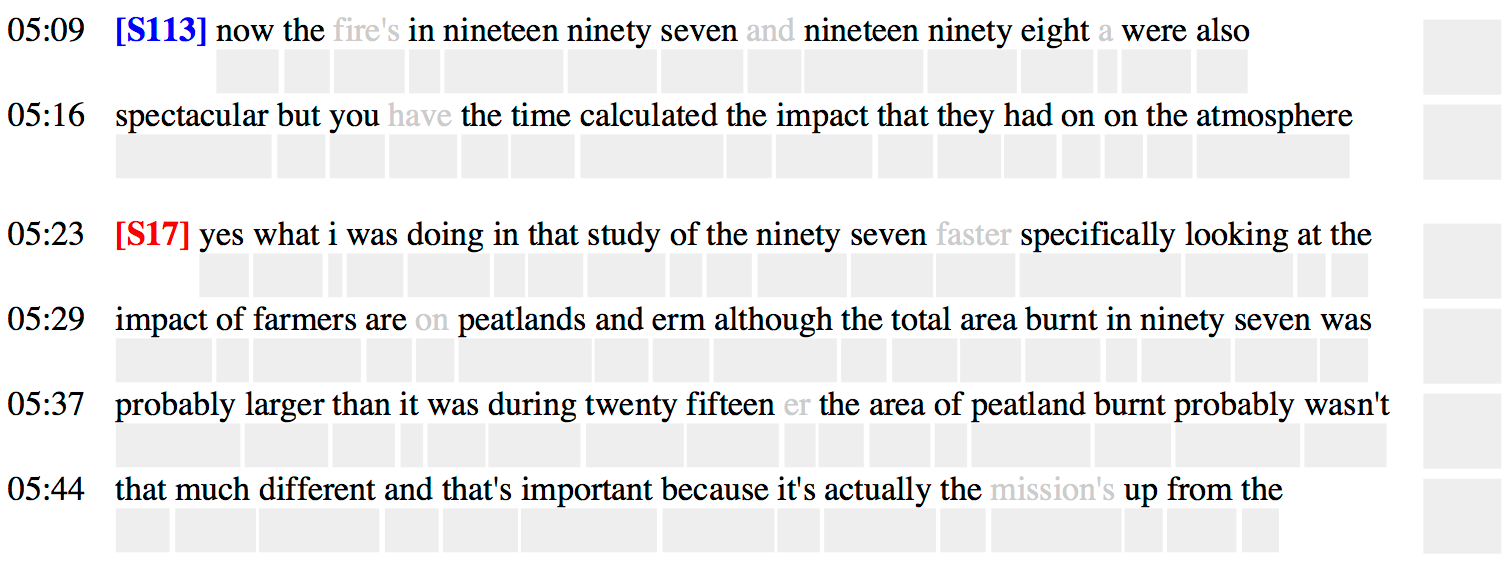
\includegraphics[width=\columnwidth]{figs/paper-prototype-design}
  \caption{Design of the paper prototype}
  \label{fig:paper-prototype-design}
\end{figure}

The transcript was generated using an automated speech-to-text system, which contained ocassional errors. We chose to
use this rather than a perfect transcript as we wanted to use automated transcription for the final system, and
removing the errors may affect user behaviour.

% Limitations of Anoto system, used normal pen for prototype
The Anoto Live Forms platform, which we used to create our system, works by dividing the page into rectangular active
zones.  When a digital pen draws inside one of these zones, that data can then be captured digitally and processed.
Traditionally this is used to detect when someone has ticked a box on a form, or to extract an image of a signature
drawn inside of a box.  To capture edit annotations that linked to the text of the transcript, we designed our layout
to use rectangular active zones that aligned with the location of each word.

% Edit commands: selector beneath word (double-spaced) and at end of line, removal by crossing word
From what we had witnessed from previous experiments, the most common annotations producers used were underline,
strikethrough and drawing a line down the side of the page.  To capture strikethrough, we drew an invisible active zone
on top of each word, so that when a line is drawn through the word, the zone is triggered. For underline, we draw a
shaded active zone directly below each word, so that drawing a line underneath a word triggers the zone. The transcript
was printed double-spaced to leave enough room for these boxes. Finally, we draw a shaded active zone at the end of
each line. Drawing a line through this zone would select the whole line.

% Additional features: paragraphs and speaker ID with gender, timestamp at start of line, confidence shading
The speech-to-text system we used provided additional information with the transcript.  Each word came with a timestamp
and a confidence rating. We wrote the timestamp at the beginning of each line in \textit{MM:SS} format, and used
confidence shading to grey-out lower confidence words.  The speech-to-text system also used speaker diarization
techniques to segment the transcript by speaker. This provided a speaker label and estimated gender for each segment.
We used paragraphs to segment the transcript, and wrote the speaker label at the start of each paragraph. We used blue
colouring for male speakers, and red for female speakers.

\subsection{Evaluation method}

%TODO Explain interview protocol and analysis

%TODO Why are participants asked to adopt three different strategies?

%TODO Explain design decisions, e.g. double-spacing, confidence shading

To evaluate our paper prototype, we ran a short experiment in which radio producers used our inactive prototype to
annotate real transcripts as if they were editing them.  We asked them to edit the transcripts in different ways, and
interviewed them afterward to compare the various approached. Producers are very busy, so to gain enough participants
in the time we had available, we designed the experiment so it could be completed within an hour.

We recruited five producers by using the contacts that we made from previous experiments. Two of the participants
worked in current affairs, two in science and one in documentaries.  The participants had between 7 and 13 years
experience working as a radio producer.

For the transcript, we asked each participant to provide us with a recent interview they had made, which we ran through
our speech-to-text system. We used this automated transcript for each participant's experiment so that they were
working with authentic speech, and a transcript that would be the same as that from a working system.

To help explore our questions about annotation and editing gestures, we directed participants to employ three different
strategies when using the prototype. This forced them to experience different ways of interacting with the prototype,
which they could later reflect on and compare. We instructed them to follow these directions for the first three
pages of their transcript: 

\begin{itemize}
  \item \textit{Page 1}: Undirected\\Edit the speech by annotating the transcript as you would normally.
  \item \textit{Page 2}: Underline only\\Edit the speech only by underlining words that you want to keep.
  \item \textit{Page 3}: Strikethrough only\\Edit the speech only by putting a line through words you don't want to keep.
\end{itemize}

The `undirected' strategy allowed us to see what gestures producers currently use, or want to use, without being
influenced by the design of the prototype or constrained by its limitations. We included the underline and
strikethrough strategies as we believed these to be the two most commons approaches, and we wanted the participants to
compare them directly.

We were also interested in learning about additional features and their value. To get feedback on the value of speaker
diarization, we produced two versions of each participant's transcript -- one with speaker diarization and one without.
The speaker information was used to segment the transcript into paragraphs, and the start of each paragraph was
labelled with the speaker identifier in square brackets (e.g.  \texttt{{[}S1{]}}).  For \textit{Page 4}, each
participant was presented with a transcript that included speaker diarization, and asked to edit the speech by
annotating the transcript any way they wished.

Timestamps, line selection and confidence shading were included with all of the prototypes. For these features, we
chose not to produce versions with/without as participants should be able to judge their value without having to see
them removed. Producing different versions for each would also unduly lengthen the experiment.

At the end of the test, we conducted a semi-structured interview with each participant. The following questions were
asked, but we also let the participants talk about whatever else they wanted to.

{\singlespacing
\begin{itemize}
  \item How do you normally use a pen to edit the transcript?
  \item Do you prefer to select parts you want to keep, or remove parts you don't want to keep?
  \item Which features of the prototype did you find useful?
  \item Were there any features missing that you would want added?
\end{itemize}
}

The experimenter wrote down the participants responses from the interview. These were then categorised into natural
gestures, edit gestures and additional features. We counted the frequency of each response within the categories to
see how popular the different approaches and features were. The participant's annotated transcripts were also
collected.

\subsection{Results}
The reaction to the system was overwhelmingly positive. All of the participants could immediately see the value of such
a system and most remarked that it would save them significant amounts of time and \textit{``revolutionise''} their
production workflow.

\subsubsection{Natural gestures}

The participants started the experiment by editing the transcript using any gestures they wanted.
Table~\ref{tab:natural-gestures} lists the gestures that were used, and by which participants.

\begin{table}[ht]
  \centering
  \begin{tabular}{|l|c|c|c|c|c|c|}
    \hline
                            & P1        & P2        & P3        & P4        & P5        & Count \\
    \hline
    Underline               & $\bullet$ & $\bullet$ & $\bullet$ & $\bullet$ &           & 4 \\
    \hline
    Strikethrough           & $\bullet$ & $\bullet$ &           & $\bullet$ & $\bullet$ & 4 \\
    \hline
    Line down side          & $\bullet$ & $\bullet$ & $\bullet$ &           & $\bullet$ & 4 \\
    \hline
    Comments                & $\bullet$ & $\bullet$ &           &           & $\bullet$ & 3 \\
    \hline
    Correction              & $\bullet$ &           &           &           & $\bullet$ & 2 \\
    \hline
    In/out marks            & $\bullet$ &           &           & $\bullet$ &           & 2 \\
    \hline
    Scribble-out mistake    &           & $\bullet$ & $\bullet$ &           &           & 2 \\
    \hline
    Lasso                   &           &           &           &           & $\bullet$ & 1 \\
    \hline
    Line through paragraph  &           &           &           &           & $\bullet$ & 1 \\
    \hline
  \end{tabular}
  \caption{Natural gestures used by each participant to edit their transcripts}
  \label{tab:natural-gestures}
\end{table}

\begin{figure}[h]
  \centering
  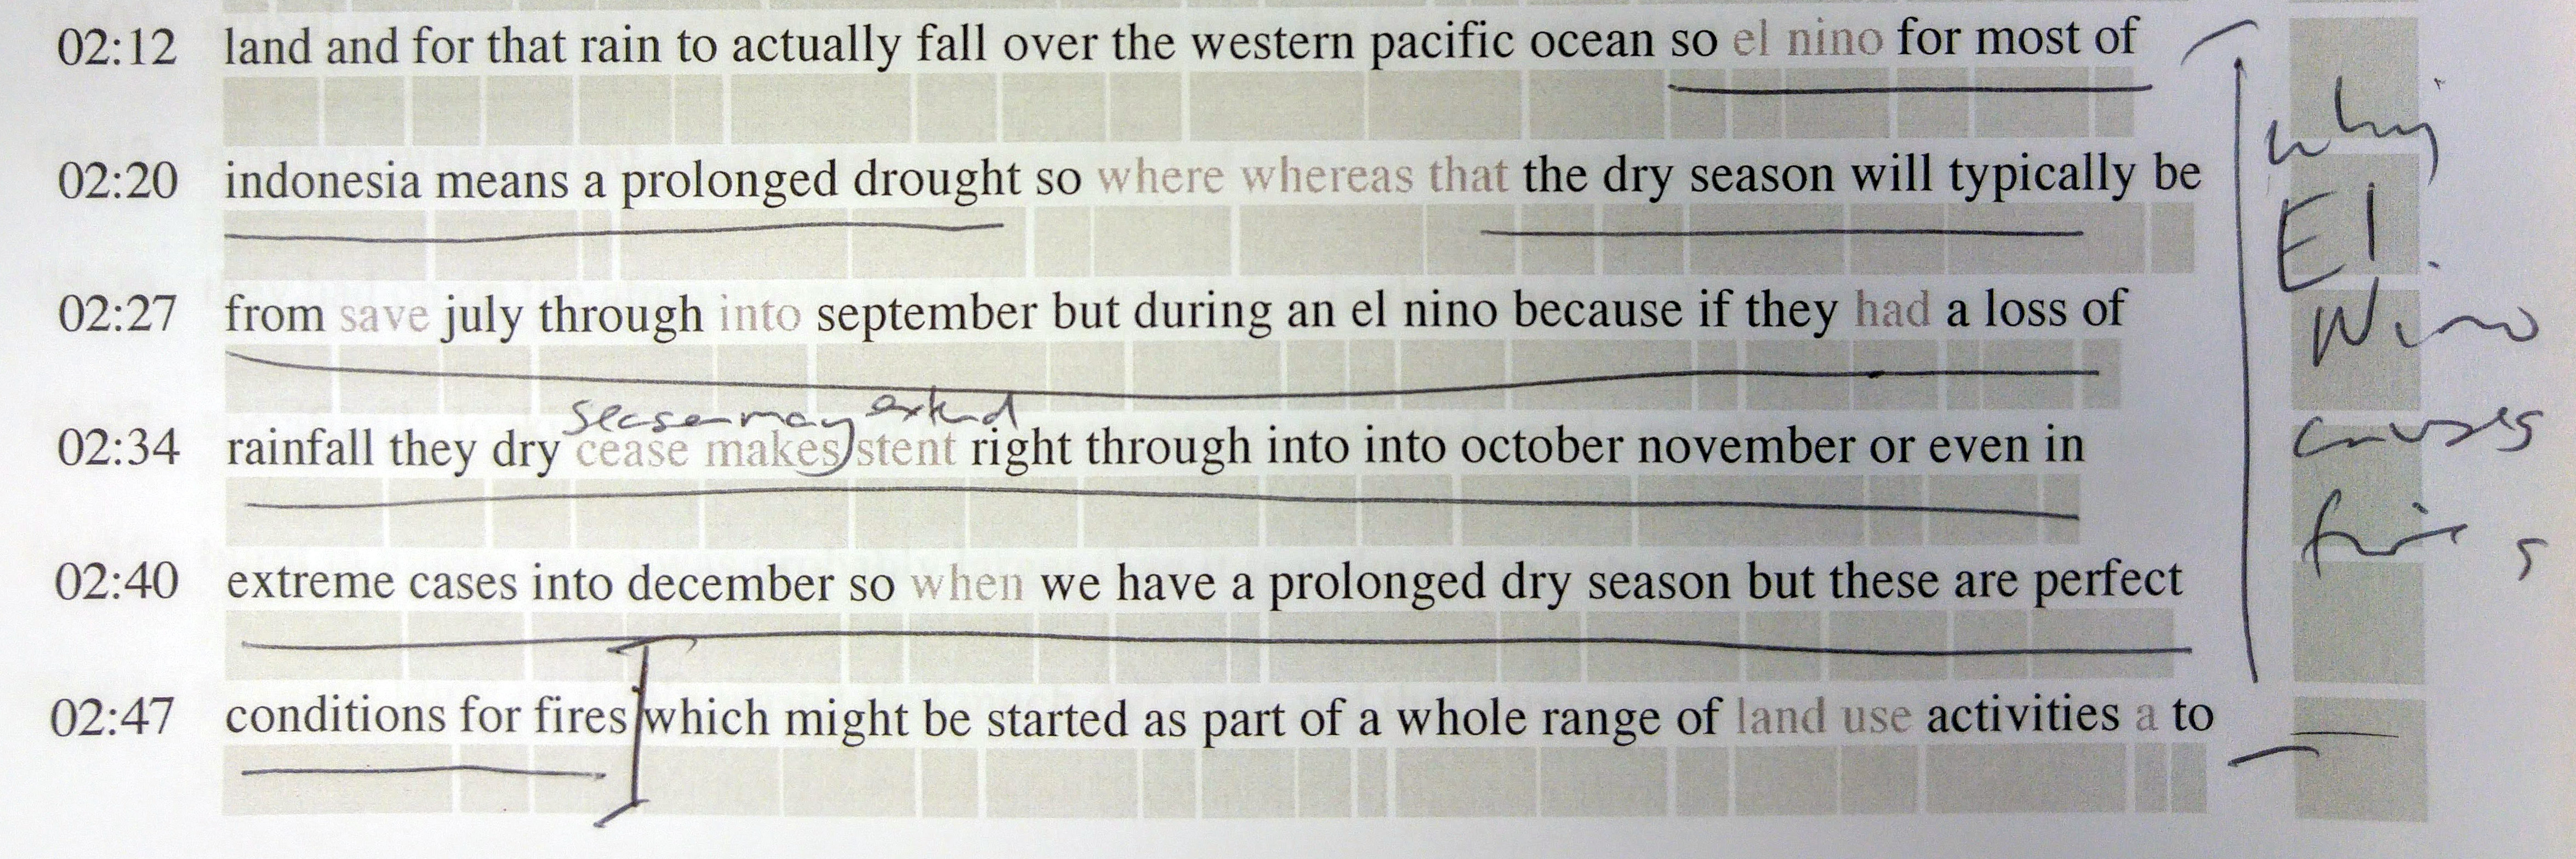
\includegraphics[width=\columnwidth]{figs/mockup-cropped}
  \caption{Paper prototype with natural annotations, including
    underlining, line down the side with notes, word corrections, and a
    vertical line to indicate the end of an edit.}
  \label{fig:natural}
\end{figure}

Four different gestures were used to select content -- underline, line down side, in/out marks and lasso.  Underline
was used by all participants but one, who was mainly interested in deleted unwanted content.  Drawing a line down the
side was used by three participants, as it is quicker and more efficient than underlining for selecting large chunks of
material.  Some participants combined both by using underline to be more precise about the start and end of their
selection.  One of the participants made a mistake when underlining, so scribbled out the underline to undo it.

`In/out marks' refers to drawing short vertical or diagonal lines before and after the words of a selection. These
indicate the in- and out-points for edits. One participant drew an analogy between these marks and the splicing of
magnetic tape, which was how radio programmes were edited before the digital age. `Lasso' refers to selecting a number
of words by drawing a line around them.

Two gestures were used to delete content -- strikethrough and drawing a line through a paragraph. These parallel the
underline and line down side gestures that are used for selection, but instead involve drawing a line through the words
themselves.
%TODO Expand

Finally, two participants corrected mistakes in the transcript by writing the correction over/above the
word, or to the side of the page.
%TODO Expand

Each participant used a different mixture of annotation techniques.
%TODO Expand

\subsubsection{Edit gestures}\label{sec:paper-proto-edit-gestures}
We asked each participant whether they preferred selecting or deleting words for editing the transcript.  P1, P3 and P4
reported that they preferred selecting, P1 commented that it \textit{``felt more natural''} to them and P4 said
deleting felt \textit{``counter-intuitive''}.

P2 and P5 reported that they preferred deleting words. P2 commented that \textit{``the challenge is to nibble away''}
and it was \textit{``the way my brain works''}. P5 said they prefer to \textit{``get stuff out of the way''}.

All of the participants were certain about which they preferred, but there was no overall consensus. Additionally, we
can see in Table~\ref{tab:natural-gestures} that all participants used a mixture of select and delete gestures during
the undirected annotation.

\subsubsection{Additional features}

% speaker diarization
Four of the five participants said that they found the paragraphs and speaker information useful. Typically, interviews
are recorded with a presenter and contributor, and the participants said they found it valuable to know when the
presenter is asking a question. Three of the participants said that they were able to find the questions much more
easily with this feature enabled. However, P2 said they found the speaker diarization to be \textit{``distracting''},
particularly when it was inaccurate.

% timestamps/confidence shading
All participants found the timestamps and confidence shading features useful, but P2 said that the timestamps are
\textit{``not needed on every line''} and P5 suggested that one timestamp per page would be sufficient. All of the
participants liked being able to select whole lines at a time. P5, who prefers to remove words, asked whether a similar
function could be available to delete content.

\subsubsection{Missing features}

During our testing, some participants suggested adding features that were not included, or used the prototype in a
way it was not designed.
% highlighting
P3, P4 and P5 remarked that they often highlight important bits of transcripts, usually with asterisks or stars.
P1 and P3 also suggested that the underline gesture could be extended so that underlining words twice marks them as
being more important.

% labelling, margins
Three participants made notes on the side of the page to label their content or to make a note for themselves. Due to
the limited space, the notes were often scrawled sideways in small writing. If the prototype was active, writing notes
on the transcript itself would likely have triggered the active zones located on and below each word. This would cause
the user to inadvertantly create edits to the audio. P3 suggested that it may be worth adding a margin. Providing an
inactive margin would give users a `safe space' to make freehand notes without editing the audio.

% correction
Two participants corrected words in the transcript by writing over or above the incorrect word. As the transcript was
double-spaced, there was just enough room between lines to write the correct word in small writing.
% listening/playback
P3, P4 and P5 expressed a desire to listen to the audio while reading/editing it, which echoes the importance of
listening noted in Chapter~\ref{chp:screen}.

%- Useful to know where presenter is asking question

%Diarization
%- Neal found it easier
  %- Shows where the questions are
%- Phil found it distracting
%- Wes found it absolutely useful
%- Marnie 'made it much easier', liked having paragraphs (usually one point per
%paragraph)


%Timestamps
%needed every couple of minutes

%Use L/R channels for presenter/contributor
%- Phil and Wes
%- Sometimes multiple on R channel (about one in eight interviews)

%Prefer landscape to portrait (landscape is `irritating' and doesn't match
%what's on screen)

%Whole line
%- Would like to delete line at a time

%Note-taking
%- One doesn't take many notes

%Correction
%- One corrects then selects edits
%- Wes would like option

%Highlighting
%- Asterix/star to mark important bits (Phil, Neal)
%- Underline twice (Neal, Marnie liked idea)
%- Wes sometimes double-stars

%Delete vs select (2 vs 3)
%- Phil likes to `get stuff out of the way'
  %- Words that aren't marked should be kept by default
  %- Underline should undo delete
%- Neal prefers selecting over deleting
  %- Delete should undo select, if underlined too far
%- Wes prefers selecting - deleting is `counter-intuitive'
  %- Would like delete to override select, but would like options for opposite
%- Marnie found it trickier to delete than select, selection is more natural
  %- worried about deleting something good
%- Alex feels delete is more natural, 'way may brain works, 'challenge is to
%nibble away', thinks delete should be active, select should override delete

%Margin
%- Phil wouldn't need a margin
%- Neal would like one

%Export
%- gaps should be put between edits (real-time?)

%Transcript
%- Phil and Neal no problems
%- Wes had problems (strong Scottish accent) made it unusable

%Observation
%- Neal
  %- underlined as he read (unprompted), scribbled out when mistake made
  %- found it more difficult to only delete
%- Wes
  %- vertical lines for in/out points

%Other
  %- Neal would like to press and hear word (on laptop?)
    %- Wes: Don't know what sounds good
  %- Wes works in a team of 3/4. They use Box to collaborate
  %P4 reported that they usually work in teams of 3 or 4 people. They use Google Docs to collaborate on a central
  %programme script, so they can all edit the document simultaneously.

\subsection{Discussion}

In this section, we set out to answer three questions about the gestures producers use to edit printed transcripts, and
which features we should include in our paper-based audio editing interface. We did this by evaluating a paper
prototype of our interface on five radio producers using real content.

  %\item What gestures are currently used by radio producers to annotate transcripts?
  %\item Do producers prefer to select content they want to keep, remove content they don't want, or a mixture of the
    %two?
  %\item Which additional features (e.g. timestamps, speaker labelling, confidence shading) should be included in the
    %layout?

We observed that the participants used a variety of gestures to select and delete content, with underline,
strikethrough and a line down the side being the most common.  This confirms our assumptions about these being the most
popular annotations, which drove the design of our prototype.  The other gestures included in/out marks and lasso for
selection, and drawing a line through a paragraph for deletion.  In \citet{Weibel2008}, strikethrough was also used for
delete, but something similar to in/out marks was used for annotating a specific region.

There were mixed but strong opinions on whether it was better to select good content or remove bad content.  Most
participants used a mixture of both approaches when undirected. Given the lack of consensus, it would be best to give
producers the option to do both, but this raises the issue of what should happen when a word is both selected and
deleted.  If one overrides the other, then it could function as an undo mechanism. The more conservative approach would
be for selection to override deletion, so that speech can always be recovered. However the system does not delete any
audio, so this is not a risk.

Selection and deletion could be used together at different scales, where one is used to select/delete large chunks,
then the other is used to refine the choise by selecting/deleting smaller words or chunks within the larger ones. In
our results, we saw that selecting large chunks is more popular than deleting large chunks. Also, there is likely to be
more interest in removing individual words, such as for `de-umming', than there is for selecting individual words. For
this style of use, it may be better for delete to override select.

When underline is used to select content, it implies that everything else should be discarded except for the underlined
parts. Alternatively, underline could be used to highlight parts of interest. In a later stage, the user could then
choose to either keep everything except the deleted words, or to keep only the highlighted words minus the deleted
words. This would give greater flexibility to different modes of use, like we saw in
Section~\ref{sec:paper-proto-edit-gestures}.

Most participants valued the additional features we tested -- speaker diarization, timestamps and confidence shading,
but reported that timestamps on every line are unnecessarily frequent. During our testing, we also identified missing
functionality for labelling, correction, highlighting and playback.

% Missing features
Handwritten text was also used to make
corrections to the transcript, and to label parts of the transcript.

% labelling
Three participants made notes on the side of the page to label their content or to make a note for themselves. Two of
the participants remarked that there was no free space in which to make notes, and suggested that it may be worth
adding a margin. Writing notes on the transcript itself would trigger the active zones that are on and below each word.
Providing an inactive margin would allow users to make freehand notes without inadvertantly making edits to the speech.

% correction
Two participants corrected words in the transcript by writing over or above the incorrect word. 
Potentially users could write the replacement word in an active zone, but...

% highlighting
Most participants remarked that they normally mark important bits of the transcript, often with asterisks or
stars. Underlining twice could also introduce a two-tier selection system.
Possibly the side boxes could be used to rate or star a selection.

% playback
Some participants expressed a desire to listen to the media from the paper interface, and this functionality has been
shown to be useful in previous work. %TODO Reference
An external device, such as a phone, computer or portable media player could be used to replay the audio while using
the paper interface.

Users could start playback by pressing a word with the digital pen. This could be
achieved either by wirelessly linking the digital pen to a computer that plays the content, or by storing the audio on
the pen itself similarly to the LiveScribe Sound
Stickers\footnote{\url{http://store.livescribe.com/sound-stickers-1-1.html}}.

% natural annotation:
% underline, strike and line down side most used, reinforced design decision
% comments and correction were popular, no space to write them
% in/out marks, lasso also used for selection, line through paragraph used for deletion, but to lesser extent

% edit gestures:
% no consensus on best approach, both used when naturally annotating, so both should be available
% what to do when using both? underline override strike or vice-versa?

% additional features:
% speaker diarization - yes
% timestamps - yes, but less frequently
% confidence shading - yes


%Our system performs the same function as these systems, but uses a paper
%interface rather than a screen-based one.
%Our system
%similarly interprets the paper annotations and applies them to the media
%content.
%Our system does not yet have the ability to replay content from the
%paper interface, but this is a feature that could later be included.
%Our system is based on printed transcripts rather than video frames on
%a tablet, but approaches the same problems from a different angle.
%These systems do not provide the user with any pre-written notes.
%Our system uses speech-to-text to generate a transcript, which the user can
%then annotate further.
The participants used a variety of techniques to annotate the transcripts, but underline, strikethrough and lines down
the side were common. There were strong but mixed opinions on whether selection of desired material, or removal of
unwanted material, was the best approach to use for editing, so we decided to make both options available.

%TODO What happens when underline and strike same word?

\section{System design}\label{sec:paper-design}

%TODO Why are some desired features not included, e.g. vertical lines for in/out, lasso

%TODO How are the results of the edit presented back to the user?

%TODO Underline/strikethrough interaction


Using the feedback gathered from our requirements gathering, we designed and created a working prototype of the system
(see Figure~\ref{fig:diagram}). To build our system, we collaborated with Anoto who are the manufacturers of the
digital pen. Anoto developed a system that generated the print-out and procesed the annotations. We then integrated
these system with our screen-based semantic speech editor, which includes speech-to-text and EDL generation.

\subsection{Paper interface}

\subsubsection{Design decisions}

We chose three methods for selecting and deleting material - underline, strikethrough and line down the side. Underline
represented a highlighted region which can be used to select desired material. Along with line down the side.  We did
not include in/out marks, lasso or drawing a line through a paragraph as these were not as popular, and were harder to
detect using the Anoto Live Forms system.

We chose to use speaker diarization and confidence shading, as the majority of participants in the paper prototype
wanted to keep it.  We also chose to keep timestamps, but reduced the frequency of them to once per paragraph, rather
than on every line.

We added a margin to allow users to write freehand notes without accidentally editing the audio. This was done by
drawing a rectangular area on the right side where no active zones are present.

We did not include any correction functionality as it would get confused with the edit functionality. Additionally, it
would be difficult to distinguish between edit gestures and words written as corrections.

We did not include any linked playback features as the system we were using did not support live wireless link to the
computer.

To integrate the pen system with the audio editing functionality, we integrated it with a screen-based interface. The
screen was used for asset management, including uploading new content and printing the transcript, and for
viewing/changing the edits made using the pen, and exporting the resulting audio or edit decision list.

For the line down the side selection, we opted to draw a long rectangle from the top to the bottom of the page, as this
made more sense than individual square boxes, which did not align as well with how the participants used the paper
prototype.

For the margin, we did not process any of the information so as to let the users work freehand.

To include audio editing functionality with the pen system, we integrated it with a screen-based interface. The screen
was used for asset management, including uploading new content and printing the transcript, and for viewing/changing
the edits made using the pen, and exporting the resulting audio or edit decision list.

For the line down the side selection, we opted to draw a long rectangle from the top to the bottom of the page, as this
made more sense than individual square boxes, which did not align as well with how the participants used the paper
prototype.

For the margin, we did not process any of the information so as to let the users work freehand.

Based on the feedback from users, the timestamps, paragraphs, speaker information and confidence shading have been
retained. However the timestamps only appear at the start of each paragraph. An optional margin has also been added to
allow users to make unstructured notes using their digital pen.  It is not currently possible to select a whole line at
a time, but this will shortly be added.

For each word in the transcript, two rectangular active areas are defined on the page -- one around the word itself and
another in the space directly below the word, which is lightly shaded. Any marks made on or below the word label that
word as `deleted' and `selected', respectively. This allows the user to use a digital pen to delete words using a
strikethrough, or to select words by underlining.  The annotations are automatically uploaded in batch to the system
when the pen is docked.

\subsubsection{System integration}

\begin{figure}[ht]
  \centering
  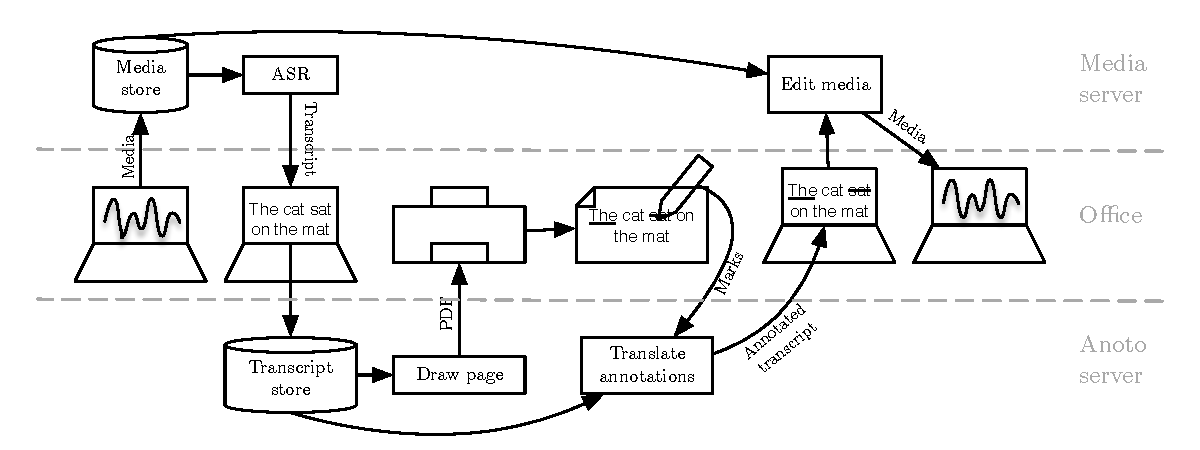
\includegraphics[width=0.5\columnwidth]{figs/uist-sys-diagram}
  \caption{System diagram, flowing from top to bottom}
  \label{fig:diagram}
\end{figure}

\subsubsection{System description}

\begin{figure}[h]
  \centering
  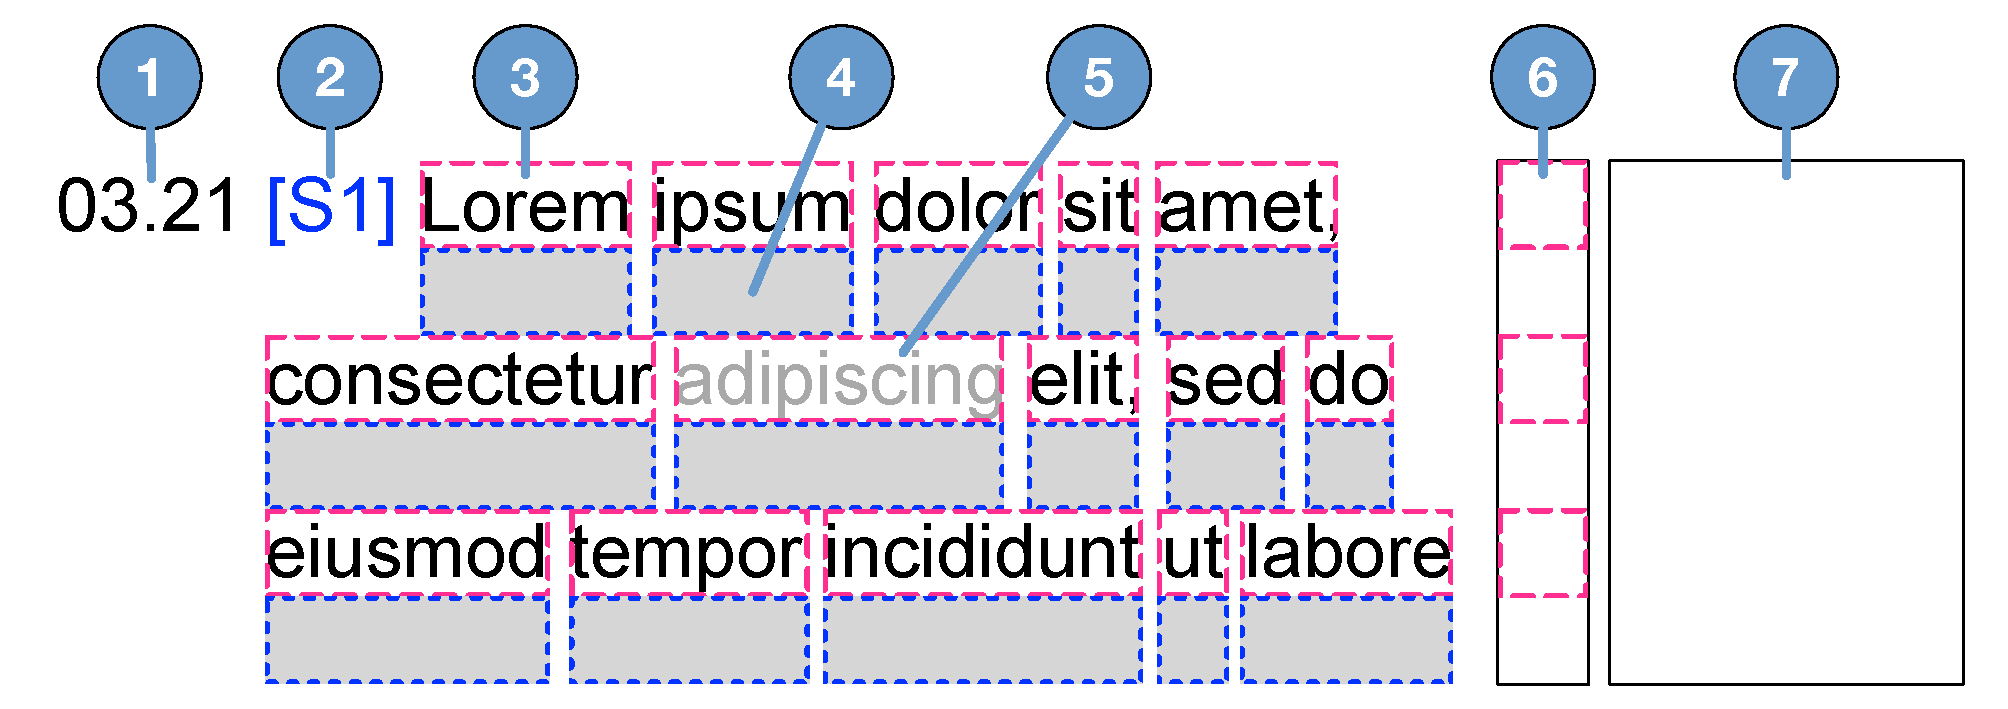
\includegraphics[width=\columnwidth]{figs/paper-interface-diagram.pdf}
  \caption{Diagram of paper interface layout with numbers features. Dotted lines indicate hidden active zones. 1:
    Timestamp at beginning of each paragraph, 2: Speaker diarization, 3: Word selection, 4: Word removal, 5: Confidence
    shading, 6: Line selection, 7: Margin for freehand notes}
  \label{fig:paper-interface-diagram}
\end{figure}

\begin{figure}[h]
  \centering
  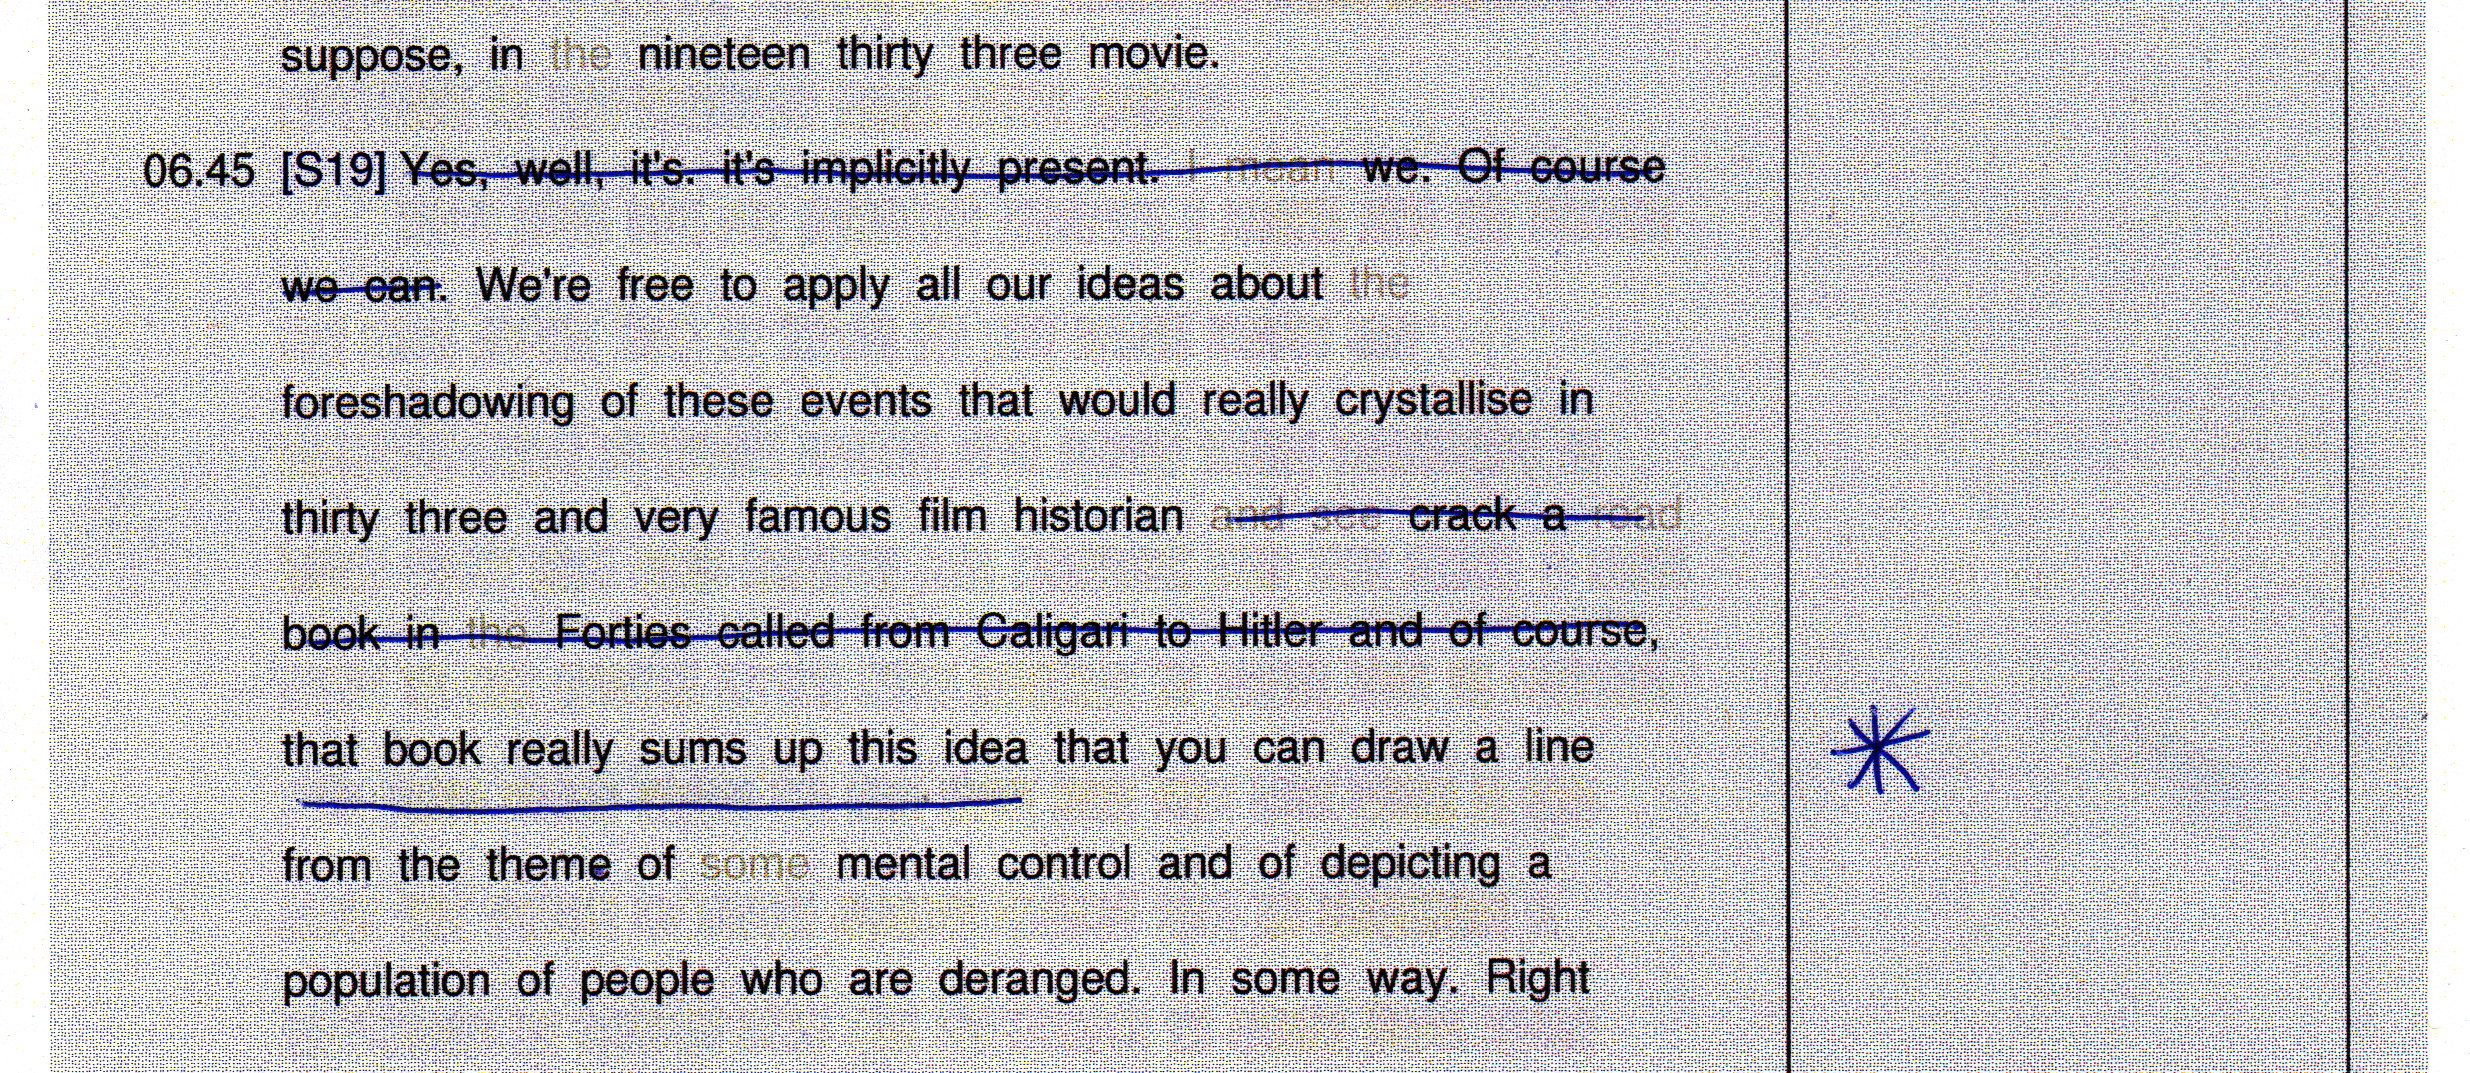
\includegraphics[width=\columnwidth]{figs/interface-darkened}
  \caption{Example of working prototype, showing the shaded box beneath each
    word, paragraph for each speaker with timestamp (06.45) and identity (S19),
    and optional margin for freehand annotations.}
  \label{fig:layout}
\end{figure}

The uploaded annotations are combined with the word timings to calculate the edit commands.  These can be used to
directly edit the media (as shown in Figure~\ref{fig:diagram}) which removes the unwanted parts of the content. This is
known as a `destructive' edit.  Alternatively, the edit commands can be used to create an edit decision list (`EDL').
An EDL file describes the in- and out-point for a series of edits, which can be loaded into audio or video editing
software.  As it is `non-destructive', this approach allows the user to make corrections to the edit before it is
rendered. 

%Several approaches can be taken in interpreting the delete and
%select annotations:
%\begin{itemize}
  %\itemsep0em
  %\item Remove words marked as deleted, except those marked as selected
  %\item Only keep words marked as selected, except those marked as deleted
  %\item Remove words marked as deleted, highlight words marked as selected
%\end{itemize}

\subsection{Screen interface}

\subsubsection{Design decisions}

\subsubsection{System description}

\begin{figure}[ht]
  \centering
  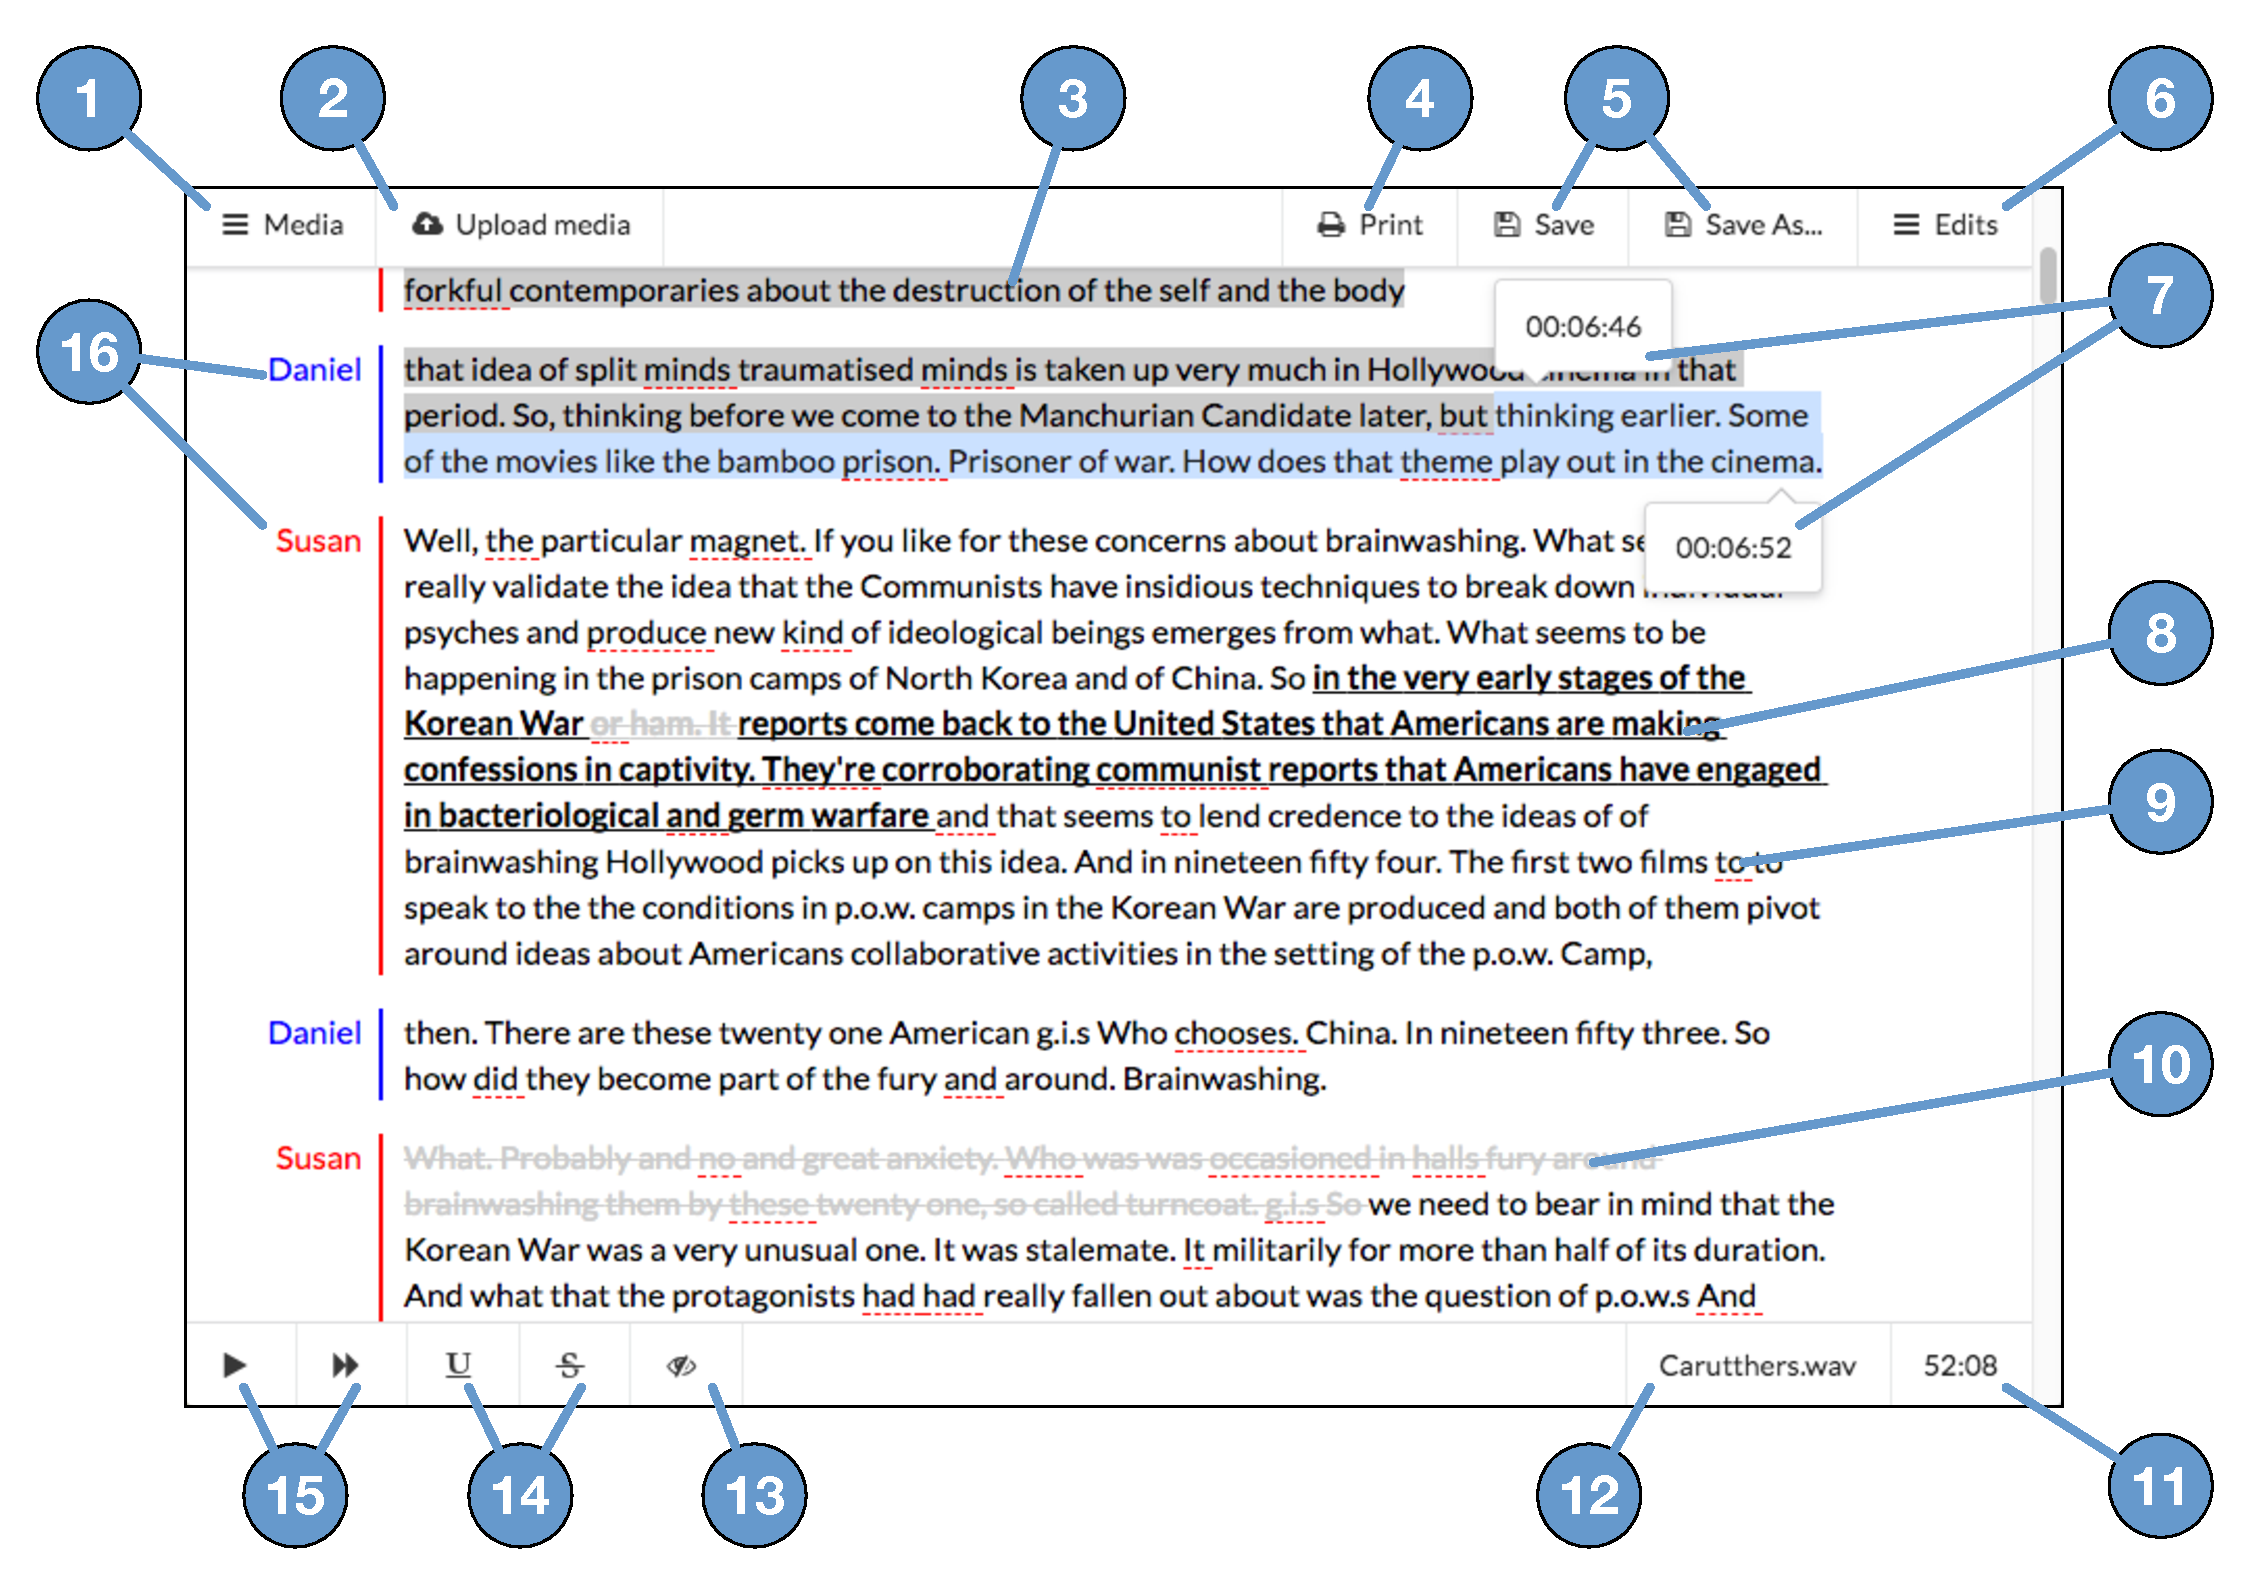
\includegraphics[width=\columnwidth]{figs/discourse-interface-labelled.pdf}
  \caption{Layout of the screen interface, with numbered features.
  1: Media storage,
  2: Media upload,
  3: Highlight current playback position,
  4: Print transcript,
  5: Save edits and corrections to transcript,
  6: Edit storage and export,
  7: Display timestamps of selection,
  8: Underline transcript,
  9: Confidence shading,
  10: Strikethrough transcript,
  11: Duration of edited audio,
  12: Name of current asset,
  13: Show/hide strikethrough,
  14: Underline/strie buttons,
  15: Playback buttons,
  16: Speaker diarization}
  \label{fig:dialogger-interface}
\end{figure}

\section{Evaluation method}\label{sec:method}

\subsection{Design and procedure}

% Explain why video recording wasn't used

\paragraph{Stage 1: Training and usability study}
Firstly, the participant will be briefed on the background, objectives and design of the study as detailed in the
protocol.  Should they wish to participate, they will be asked to read and agree to the consent form.

There are two objectives to the training stage – firstly to introduce the participant to the prototype system so that
they understand its capabilities, and secondly to test the usability of the interface.

The experimenter will set the participant up on the prototype system, including giving them access to the web-based
interface, giving them a digital pen and configuring the pen’s docking system. The participant will then receive
training on how to operate the web interface, print out transcripts correctly and use the pen.

The participant will then be asked to perform a series of typical tasks. They can ask questions and, if they
become stuck, the experimenter can prompt them. However, the experimenter will not give any other directions. The
experimenter will note whether the participant was able to successfully complete the task and document any problems or
confusion experienced during the execution of the tasks. This process will help to flag any obvious stumbling blocks.

\paragraph{Stage 2: Observation}

This stage will involve observing the participant editing two pieces of content - one using the screen-based interface
and the other using the paper-based interface. The order of the observation will be alternated between participants.
The two pieces of content should be similar in nature, but different so that the participant isn't already familiar
with the content.

The observation will be done passively to allow natural interaction with the system in the participant's normal work
environment. The experimenter will sit beside them making written notes. When the participant has some 'down-time', the
experimenter may choose to ask some questions in order to verify or clarify something they have observed.

The specific items of interest at this stage include:
\begin{itemize}
\item Editing workflow
\item Tools used
\item Data generated
\item Usability challenges and problems
\item Navigation and edit actions
\item Time taken to complete tasks
\item Unexpected reactions
\item Unanticipated usage
\end{itemize}

The prototype will be configured to electronically log the actions of the participant, which will help provide insights
into usage of the various features of the prototype.

Software Usability Scale \citep{Brooke1996}
Perceived Usefulness \citep{Davis1989}

With the participant's permission, photos may be taken of paper notes, annotations or the work environment (see 'data
protection' section below).
{\singlespacing \begin{itemize} \item Using this system in my job would enable me to accomplish tasks more quickly.
  \item Using this system would improve my job performance.
  \item Using this system in my job would increase my productivity.
  \item Using this system would enhance my effectiveness on the job.
  \item Using this system would make it easier to do my job.
\end{itemize}}

{\singlespacing
\begin{itemize}
  \item I would find this system useful in my job.
  \item I think that I would like to use this system frequently.
  \item I found the system unnecessarily complex.
  \item I thought the system was easy to use.
  \item I think that I would need the support of a technical person to be able to use this system.
  \item I found the various functions in this system were well integrated.
  \item I thought there was too much inconsistency in this system.
  \item I would imagine that most people would learn to use this system very quickly.
  \item I found the system very cumbersome to use.
  \item I felt very confident using the system.
  \item I needed to learn a lot of things before I could get going with this system
\end{itemize}
}

\paragraph{Stage 3: Interview}
Following the observation stage, the participant will be left with access to the prototype system for at least a
further week. This will give them the opportunity to use the system as part of their day-to-day work and uncover issues
which may be appear in the observation.

After this period has passed, the participant will be interviewed about their experience. The primary objective is to
compare the two production methods and extract the advantages and disadvantages of both.

An audio recording will be made of the interview (see 'data protection' section below). This will allow the participant
to speak their mind and allow the experimenter to give the participant their full attention whilst capturing all of the
provided information.

The questions asked will include:
\begin{itemize}
\item Which aspects of the screen-based system did you / did you not find useful?
\item Which aspects of the paper-based system did you / did you not find useful?
\item Overall, which system did you prefer and why?
\end{itemize}


\subsection{Participants}
To make the most of the principal investigator's position in the BBC, participants will be recruited exclusively from
the BBC. They will be invited to volunteer by way of email passed around using existing contacts in various departments
that produce speech-based content. 

The nature of the study requires that participants conduct the tasks as part of their day-to-day job. Therefore,
participants will be required to gain permission from their line manager to take part.

Programmes and producers vary significantly in genre and production techniques.  To take this into account,
participants will be recruited so that there is a representative range of styles.

The participants had between 8 and 28 years experience of professional radio production, with a mean average of
16 years experience.

\subsubsection{Selection criteria}

\begin{itemize}
\item The programme being created should be speech-based.
\item The content of the programme must not contain any sensitive material, as the transcription will be sent to a
  third-party for transcription (see 'data protection' section below).
\item The turn-around time of the programme must be long enough to allow time to recover from any technical issues
  without affecting broadcast output.
\item The participant must have permission from their line manager to take part.
\end{itemize}

The study will involve between six and nine participants, depending on how many meet the criteria. This should uncover
over 90\% of usability problems \citep{Nielsen1993} whilst covering a range of genres and styles, and being a
manageable number given the duration of the experiment.

The study will take place at the participant's own desk at their normal place of work. As the prototype is web-based,
they can use their own computer. There is a standard configuration for BBC desktop computers, so the environment should
be similar for each participant. Use of display screen equipment is already covered under the existing BBC risk
assessment process.

\subsection{Analysis}


\section{Study results}\label{sec:paper-results}

\subsection{Qualitative analysis}

% MAIN TOPICS:
% Annotation
% Correction
% Editing
% Listening
% Normal workflow
% Paper admiration/restrictions/waste
% Screen-based working/reading paper
% Transcript accuracy
% Transcript itself


% OTHER TOPICS:
% Collaboration
% Cost
% Custom vocab
% Digital/analogue
% Combining recordings
% Non-linear workflow
% Pen hardwaare
% Working remotely
% Speaker diarization
% Speed
% Structuring thoughts
% Transcription speed
% Translation


\subsection{Metrics}

% Popularity
\subsubsection{Preference}

\begin{itemize}
  \item Normal paper: 2
  \item Screen: 2
  \item Pen: 4
\end{itemize}

% Usefulness and usability
\subsubsection{Usefulness and usability}

\begin{figure}[h]
  \centering
	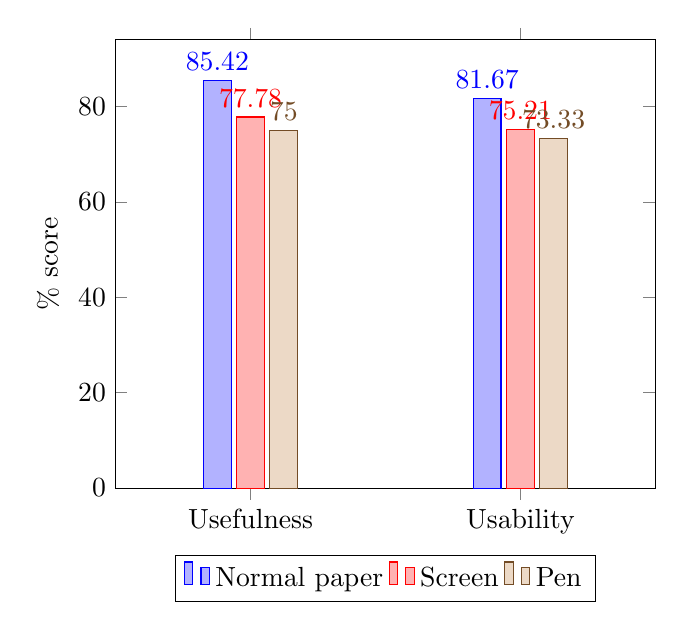
\begin{tikzpicture}
	\begin{axis}[
			ybar,
			ymin=0,
			enlarge x limits=0.5,
			legend style={at={(0.5,-0.15)},anchor=north,legend columns=-1},
			ylabel={\% score},
			symbolic x coords={Usefulness, Usability},
			xtick=data,
			nodes near coords,
			nodes near coords align={vertical},
			]
	\addplot coordinates {(Usefulness,85.42) (Usability,81.67)};
	\addplot coordinates {(Usefulness,77.78) (Usability,75.21)};
	\addplot coordinates {(Usefulness,75.00) (Usability,73.33)};
	\legend{Normal paper, Screen, Pen}
	\end{axis}
	\end{tikzpicture}
  \label{fig:usefulusable}
  \caption{Mean average scores for usefulness and usability}
\end{figure}


% Speed
\subsubsection{Speed}

\begin{figure}[h]
  \centering
  \begin{tikzpicture}
  \begin{axis}[
    legend pos=outer north east,
    legend cell align=left,
    xmin=0,
    ymin=0,
    xlabel={Audio length (mins)},
    ylabel={Edit time (mins)}]

  % NORMAL
  \pgfplotstableread{
    X Y
    30 30
    58 43
    32 23
    35 53
    28 35
    28 32
    47 62
    28 22
  }\normaltimes
  \addplot [only marks, mark = *, red] table {\normaltimes};
  \addlegendentry{Normal paper}
  \addplot [thick, red, forget plot] table[
      y={create col/linear regression={y=Y}}
  ]{\normaltimes};
  %\addlegendentry{Normal trend}

  % SCREEN
  \pgfplotstableread{
    X Y
    37 24
    61 61
    30 30
    25 49
    26 31
    41 28
    37 37
    33 45
  }\screentimes
  \addplot [only marks, mark = square*, blue] table {\screentimes};
  \addlegendentry{Screen}
  \addplot [thick, dotted, blue, forget plot] table[
      y={create col/linear regression={y=Y}}
  ]{\screentimes};
  %\addlegendentry{Screen trend}

  % PEN
  \pgfplotstableread{
    X Y
    12 9
    75 56
    31 17
    22 19
    27 27
    38 37
    33 33
    28 41
  }\pentimes
  \addplot [only marks, mark = diamond*, green] table {\pentimes};
  \addlegendentry{Pen}
  \addplot [thick, loosely dashed, green, forget plot] table[
      y={create col/linear regression={y=Y}}
  ]{\pentimes};
  %\addlegendentry{Pen trend}

  \end{axis}
  \end{tikzpicture}
  \caption{Edit time performance for each editing system, with linear regression plot}
  \label{fig:penedittime}
\end{figure}

Mean edit time, per minute of input audio:
\begin{itemize}
    \item Normal paper: 59.2 seconds (x0.9867 real-time)
    \item Screen: 59.34 seconds (x0.9890 real-time)
    \item Pen: 49.77 seconds (x0.8295 real-time)
\end{itemize}

% Usefulness


% Usability




\section{Discussion}\label{sec:paper-discussion}

\section{Conclusion}\label{sec:paper-conclusion}

\subsection{Future work}
